\documentclass[]{article}
\usepackage{float} % To get table captions at the top
\floatstyle{plaintop}
\restylefloat{table}
\usepackage[stable]{footmisc}
\usepackage{lmodern}
\usepackage{amssymb,amsmath}
\usepackage{biblatex}
\usepackage{ifxetex,ifluatex}
\usepackage{fixltx2e} % provides \textsubscript
\ifnum 0\ifxetex 1\fi\ifluatex 1\fi=0 % if pdftex
  \usepackage[T1]{fontenc}
  \usepackage[utf8]{inputenc}
\else % if luatex or xelatex
  \ifxetex
    \usepackage{mathspec}
    \usepackage{xltxtra,xunicode}
  \else
    \usepackage{fontspec}
  \fi
  \defaultfontfeatures{Mapping=tex-text,Scale=MatchLowercase}
  \newcommand{\euro}{€}
\fi
% use upquote if available, for straight quotes in verbatim environments
\IfFileExists{upquote.sty}{\usepackage{upquote}}{}
% use microtype if available
\IfFileExists{microtype.sty}{\usepackage{microtype}}{}
\usepackage{graphicx}
\makeatletter
\def\maxwidth{\ifdim\Gin@nat@width>\linewidth\linewidth\else\Gin@nat@width\fi}
\def\maxheight{\ifdim\Gin@nat@height>\textheight\textheight\else\Gin@nat@height\fi}
\makeatother
% Scale images if necessary, so that they will not overflow the page
% margins by default, and it is still possible to overwrite the defaults
% using explicit options in \includegraphics[width, height, ...]{}
\setkeys{Gin}{width=\maxwidth,height=\maxheight,keepaspectratio}
\usepackage[unicode=true]{hyperref}
\urlstyle{same}  % don't use monospace font for urls
\setlength{\parindent}{0pt}
\setlength{\parskip}{6pt plus 2pt minus 1pt}
\setlength{\emergencystretch}{3em}  % prevent overfull lines
\setcounter{secnumdepth}{0}

\title{Simulation trials for the Revised Management Procedure, including
comparisons for when density dependence acts through fecundity or
natural mortality --- Part 1.}
\author{Kelli F. Johnson and Andr\'{e} E. Punt}
\date{School of Aquatic \& Fishery Sciences, University of Washington,
Box 355020, Seattle, WA 98195-5020, USA
Contact e-mail \href{mailto:aepunt@uw.edu}{aepunt@uw.edu}}

\begin{document}
\maketitle

\section{ABSTRACT}\label{abstract}

\subsection{Two variants of the Catch Limit Algorithm, \emph{CLA} (the
original \emph{CLA} adopted by the Commission, and an alternative
version produced by Norway) are evaluated using the trials identified by
the Scientific Committee as well as additional trials that consider
density-dependence on natural mortality rather than on fecundity and
additional ways in which the environmental change could impact whale
dynamics. Results are shown for projection periods of 100 and 300 years.
and are summarized by tables of performance statistics and
`response curves'.}

\subsubsection{INTRODUCTION}\label{introduction}

The Revised Management Procedure (RMP) of the International Whaling
Commission (IWC) \autocite{iwc_2013_rmp} represents a rigorously-tested
mechanism to provide risk-averse advice regarding catch limits for
baleen whales. The catch limit algorithm (\emph{CLA}), the process used
to calculate area-specific catch limits, represents a major component of
the RMP. The \emph{CLA} was developed based on a set of
simulation trials which explored the performance of candidate
\emph{CLAs} given uncertainty in population dynamics and demographic
parameters. Before any changes can be made to the established RMP,
results from an agreed upon list of \emph{CLA} trials must be used to
highlight differences in performance between the established procedure
and the suggested replacement \autocite{iwc_2007}.

Norway stated at the 2004 meeting that it intended to develop and
propose a change to the \emph{CLA} of the RMP. Norway also proposed that
the Maximum Sustained Yield Rate (MSYR) should refer to the $1^+$
component of the population (with $MSYR_{1+} = 1\%$ as the minimum)
instead of the mature component. The revised tuning mechanism and some
simulation results were presented at the 2006 meeting, and these were
discussed extensively. The Scientific Committee established two working
groups at the 2006 meeting, which led to the MSYR review,
completed in 2013 \autocite{iwc_2013}, and the \emph{CLA} group,
which specified trials and diagnostic plots for testing amendments
to the \emph{CLA} \autocite{iwc_2007}.
Revised results \autocite{aldrin_2007} were presented to the Committee in 2007.
However, the MSYR review had not been completed so no decision was made
at that time. The MSYR review was completed in 2013 and it concluded
that the lower bound for MSYR in trials should be $MSYR_{1+} = 1\%$.

\subsubsection{METHODS}\label{methods}

\emph{Trials structure}

The Scientific Committee agreed on a set of trials that should be
conducted when a proposal were to be made for a revision to the
\emph{CLA}, to highlight the differences in performance of the
procedures (\autocite{iwc_2007}; Table 1). The IWC \autocite{iwc_2007} also proposed
that `response curve' plots be produced for MSY rates of 1\%, 1.5\%, and
4\% and the following scenarios:

\begin{enumerate}[a.]
\itemsep1pt\parskip0pt\parsep0pt
\item
  initial depletion of 0.05\emph{K}, 0.1\emph{K}, 0.2\emph{K},
  0.3\emph{K} (R trials), 0.4\emph{K}, 0.5\emph{K}, 0.6\emph{K} (S
  trials), 0.8\emph{K}, and 0.99\emph{K} (D trials);
\item
  unreported catch level (for initial depletion levels of 0.3\emph{K},
  0.6\emph{K}, and 0.99\emph{K}), where the reported catch is either
  100\%, 80\%, 60\%, 40\%, 20\%, or 1\% of the true catch; and
\item
  positive bias in survey estimates (for initial depletion levels of
  0.3\emph{K}, 0.6\emph{K}, and 0.99\emph{K}): No bias (1.0), 1.2, 1.4,
  1.6, 1.8, and 2.0.
\end{enumerate}

The tables of results and the response curve plots show how total catch,
final population size, lowest populations size,
and average annual catch variation (AAV) change as aspects of the trials are changed.
Results are not shown for the relative recovery statistic, realized protection level,
and the continuing catch statistics owing to difficulties in defining these
statistics when natural mortality is changing over time
(and because these statistics were not used to select previous RMP variants).
Population sizes are scaled by \emph{K}, except when \emph{K} varies.
In these cases, the final population size (\emph{Pf}) and lowest
minimum population size over the distribution (\emph{Pmin}) are scaled by
the population size resulting if no catch is taken in the management period.
The reported statistics are as follows:

\begin{enumerate}[a.]
\itemsep1pt\parskip0pt\parsep0pt
\item
  Total catch (TC) distribution: (a) median, (b) 5th \%ile, (c) 96th
  \%ile, and (d) mean;
\item
  \emph{Pf} distribution: (a) median, (b) 5th \%ile, and (c) 96th \%ile;
\item
  \emph{Pmin} distribution: (a) median, (b) 5th \%ile, and (c) 96th
  \%ile; and
\item
  AAV distribution.
\end{enumerate}

All trials are conducted for 100-year and 300-year projection periods
when density-dependence acts on fecundity or natural mortality
\autocite{johnson_2015_iwc1} and whether MSYR pertains to the total (1+)
or mature female component of the population. For consistency, MSYL and
the density-dependence component are assumed to pertain to the same population
component as that to which MSYR pertains.

~

\emph{Implementation}

All simulations used MANTST, a FORTRAN program, which is available from
the IWC secretariat. MANTST version 15, used here, has several options,
where options for a single base trial are shown in Appendix (Table 3).

~

\emph{Catch Limit Algorithms}

Table 4 lists the specifications for the two \emph{CLA} variants
considered.

\subsubsection{RESULTS}\label{results}

Table 5 lists the values for the performance statistics for the two
\emph{CLA} variants for the six base-case trials (T1-D1, T1-D4, T1-S1,
T1-S4, T1-R1, T1-R4) for the two simulation lengths, for whether MSYR
pertains to the total (1+) or mature female components of the population
and the two choices for density-dependence. The results for
$MSYR_{1+}=1\%$ and $MSYR_{mat}=4\%$ are the focus for additional
analyses as these choices were selected during the MSYR review.
Figure 2 \ref{fig:respcurv_base} shows response curve plots for trials ???.


\begin{center}
Table 1.

Full set of trials required to replace the current version of
the Revised Management Procedure (RMP).
\end{center}

~

\begin{table}[ht]
\centering
\begin{tabular}{lllll}
  \hline
  & Description &              & Trial &        \\
  \hline
              & & $MSYR_{mat}$ & $1\%$ & $4\%$ \\
  \hline
  T.1   & Age structured model, maturity = 7 yr         & &       &         \\
        & D=Development (initial population $0.99K$)    & & T1-D1 & T1-D4 \\
        & R=Rehabilitation (initial population $0.30K$) & & T1-R1 & T1-R4 \\
        & S=Sustainable (initial population $0.60K$)    & & T1-S1 & T1-S4 \\
        & initial population $0.20K$                    & & T1-T1 & T1-T4 \\
        & initial population $0.40K$                    & & T1-F1 & T1-F4 \\
  T.2   & Survey Bias 0.5 & & T2-D1 & T2-D4 \\
        &                 & & T2-R1 & T2-R4 \\
  T.3   & Survey Bias 1.5 & & T3-D1 & T3-D4 \\
        &                 & & T3-R1 & T3-R4 \\
        &                 & & T3-S1 & T3-S4 \\
  T.4   & Initial Population size $P_0=0.05K$ & & T4-R1 & T4-R4 \\
  T.5   & 25 years of protection prior to management & & T5-R1 & T5-R4 \\
  T.6   & Historic error in catch ($1/2$ true catch) & & T6-R1 & T6-R4 \\
  T.7   & Age at maturity = 10 yr & & T7-D1 & T7-D4 \\
        & Age at maturity = 10 yr & & T7-R1 & T7-R4 \\
  T.9   & Episodic events: $2\%$ yearly chance that population is halved & & T9-D1 & T9-D4 \\
        &                                                                & & T9-R1 & T9-R4 \\
  T.10  & $MSYL=40\%$ & & T10-D1 & T10-D4 \\
        &             & & T10-R1 & T10-R4 \\
  T.11  & $MSYL=80\%$ & & T11-D1 & T11-D4 \\
        &             & & T11-R1 & T11-R4 \\
  T.12A & $K$ doubles over management period & & T12A-D1 & T12A-D4 \\
        &                                    & & T12A-R1 & T12A-R4 \\
  T.12B & $K$ halves  over management period & & T12B-D1 & T12B-D4 \\
        &                                    & & T12B-R1 & T12B-R4 \\
  T.13  & 33 year cycle in $MSYR (141)$ & & T13-D1 & \\
        &                               & & T13-R1 & \\
        & 33 year cycle in $MSYR (414)$ & & T13-D4 & \\
        &                               & & T13-R4 & \\
  T.15  & Survey every 10 years & & T15-D1 & T15-D4 \\
        &                       & & T15-R1 & T15-R4 \\
  T.16  & $MSYR$ declines to $1/2$ its initial value        & & T16-D1 & T16-D4 \\
  T.16  & $K$ \& $MSYR$ declines to $1/2$ its initial value & & T17-D1 & T17-D4 \\
  \hline
\end{tabular}
\end{table}


~

\begin{center}
Table 2.

An example data file used to run a single trial with 400 simulations,
for when density-dependence impacts fecundity through the 1+ population.
\end{center}

~

% latex table generated in R 3.1.2 by xtable 1.7-4 package
% Mon May 11 11:22:41 2015
\begin{table}[ht]
\centering
\begin{tabular}{lll}
 MANAGEMENT PARAMETERS         CASE  T 1A-D1 
Base case &  &  \\ 
  \hline
RANDOM PARAMETERS OPTION              & OPTRAN  & 0    \\ 
  VARIABLE BIAS OPTION                  & OPTB    & 0    \\ 
  REPORTED CATCH OPTION                 & OPTC    & 0    \\ 
  PRODUCTION MODEL OPTION               & OPTMOD  & 5    \\ 
  P$>$K BIRTH CALCULATION OPTION          & OPTDK   & 0    \\ 
  DENSITY-DEPENDENCE TYPE               & OPTDT   & 0    \\ 
  STOCHASTICITY OPTION                  & OPTDET  & 0    \\ 
  SURVEY COSTS OPTION                   & OPTSUR  & 0    \\ 
  No. OF TRIALS                         & NTRIAL  & 2    \\ 
  No. OF YEARS IN SIMULATION            & NYEAR   & 100  \\ 
  No. OF YEARS OF PREMANAGEMENT CATCH   & NPCAT   & 30   \\ 
  YEARS OF PREMANAGEMENT PROTECTION     & NPPROT  & 0    \\ 
  TRUE MSYL(1)                          & MSYL    & 0.6  \\ 
  TRUE MSY RATE(1)                      & MSYR1   & 0.01 \\ 
  PREMANAGEMENT DEPLETION (1)           & DEPL    & 0.6  \\ 
  CHANGING K OPTION                     & K99     & 0    \\ 
  CHANGING MSYR OPTION                  & MSYR99  & 0    \\ 
  CHANGING MSYR STEP                    & ISTEP   & 0    \\ 
  MATURITY PARAMETER                    & MAT1    & 7    \\ 
  MATURITY SIGMA                        & MSIG    & 1.2  \\ 
  RECRUITMENT PARAMETER                 & REC1    & 7    \\ 
  RECRUITMENT SIGMA                     & RSIG    & 1.2  \\ 
  MORTALITY PARAMETER 1                 & MORT1   & 0.04 \\ 
  MORTALITY PARAMETER 2                 & MORT2   & 0.07 \\ 
  MORTALITY FUNCTION                    & MORTIP  & -1   \\ 
  MAXIMUM AGE                           & MAXAGE  & 20   \\ 
  MINIMUM AGE OF MATURITY               & MINMAT  & 0    \\ 
  EPIDEMIC RATE                         & ERATE   & 0    \\ 
  COMPONENTS (0=EXPLOITABLE; 1=TOTAL1+; 2=MATURE) &  &      \\ 
  MSYR COMPONENT                        & OPTF    & 1    \\ 
  MSYL COMPONENT                        & OPTMSYL & 1    \\ 
  DENSITY-DEPENDENT COMPONENT           & OPTDD   & 1    \\ 
  FREQUENCY OF ABUNDANCE ESTIMATES      & IFREQ   & 5    \\ 
  YEAR OF LAST SURVEY                   & ENDSUR  & 100  \\ 
  YEAR CV CHANGES                       & IYRCV   & 100  \\ 
  BIAS IN ABUNDANCE ESTIMATES           & BIAS0   & 1    \\ 
  CV OF CV ESTIMATES (1st)              & CV1EST  & 0.2  \\ 
  PROCESS ERROR PARAMETER               & ETA     & 1    \\ 
  MINIMUM No. OF DEGREES OF FREEDOM     & DOFMIN  & 5    \\ 
  STARTING VALUE FOR A                  & INITA   & 0.2  \\ 
  STARTING VALUE FOR Z                  & INITZ   & 0.2  \\ 
  DEPLETION (0:SINGLE VALUE;1:READ IN)  & OPTDPL  & 0    \\ 
   \hline
\end{tabular}
\end{table}


~

\begin{center}
Table 3.

Specification of the \emph{CLA} variants.
\end{center}

~

% latex table generated in R 3.1.2 by xtable 1.7-4 package
% Mon May 11 11:43:31 2015
\begin{table}[ht]
\centering
\begin{tabular}{lrrr}
 parameter & alt1 & alt2 & original \\ 
  \hline
PROBABILITY LEVEL (PPROB)      & 0.50 & 0.50 & 0.40 \\ 
   \hline
MIN MSY \% (PYMIN)              & 0.00 & 0.00 & 0.00 \\ 
  MAX MSY \% (PYMAX)              & 0.05 & 0.05 & 0.05 \\ 
  DEPLETION MIN (DTMIN)          & 0.00 & 0.00 & 0.00 \\ 
  DEPLETION MAX (DTMAX)          & 1.00 & 1.00 & 1.00 \\ 
  BIAS MIN (PBMIN)               & 0.00 & 0.00 & 0.00 \\ 
  BIAS MAX (PBMAX)               & 1.67 & 1.67 & 1.67 \\ 
  SCALE FACTOR (PSCALE)          & 4.00 & 4.00 & 4.00 \\ 
  PHASEOUT PERIOD (PHASET)       & 8.00 & 8.00 & 8.00 \\ 
  PHASEOUT PROPORTION (PHASEP)   & 0.20 & 0.20 & 0.20 \\ 
  ASSESSMENT CYCLE (PCYCLE)      & 5.00 & 5.00 & 5.00 \\ 
  INTERNAL PROTECTION LEVEL      & 0.54 & 0.54 & 0.54 \\ 
  CATCH CONTROL SLOPE (PSLOPE)   & 4.72 & 9.34 & 3.00 \\ 
  ACCURACY TOLERANCE (ACCTOL)    & 0.00 & 0.00 & 0.00 \\ 
  NOFRULE                        & 8.00 & 8.00 & 8.00 \\ 
   \hline
\end{tabular}
\end{table}


\begin{center}
Table 4.

Median, 5\% percentile, 96th\% percentile, and mean of the total
catch distribution for when density dependence impacts fecundity (F)
or natural mortalitly (M). All values are scaled by carrying capacity (\emph{K}).
400 replicates were performed in each case.
\end{center}

~

% latex table generated in R 3.1.2 by xtable 1.7-4 package
% Wed May 13 21:43:17 2015
\begin{table}[ht]
\centering
\begin{tabular}{llllllllllll}
  \hline
  \hline
Trial &  & Total catch &  &  & Final population size &  &  & Lowest population size &  &  & AAV \\ 
   & Med & 5\% & 96\% & Mean & Med & 5\% & 96\% &  &  &  &  \\ 
  F1-T1-R1 & 0.957 & 0.574 & 1.392 & 0.962 & 0.881 & 0.807 & 0.929 & 0.3 & 0.3 & 0.3 & 0.022 \\ 
  F1-T1-S1 & 1.76 & 0.937 & 2.265 & 1.7 & 0.782 & 0.642 & 0.932 & 0.593 & 0.6 & 0.6 & 0.023 \\ 
  F1-T1-D1 & 2.223 & 1.47 & 2.727 & 2.19 & 0.771 & 0.615 & 0.908 & 0.56 & 0.589 & 0.638 & 0.03 \\ 
  F2-T1-R4 & 1.595 & 0.649 & 2.969 & 1.663 & 0.968 & 0.858 & 0.994 & 0.3 & 0.3 & 0.3 & 0.024 \\ 
  F2-T1-S4 & 1.68 & 0.73 & 3.148 & 1.811 & 0.974 & 0.867 & 0.997 & 0.6 & 0.6 & 0.6 & 0.027 \\ 
  F2-T1-D4 & 3.615 & 1.945 & 4.704 & 3.512 & 0.88 & 0.781 & 0.969 & 0.758 & 0.778 & 0.8 & 0.026 \\ 
  M1-T1-R1 & 0.901 & 0.531 & 1.33 & 0.906 & 0.9 & 0.84 & 0.939 & 0.3 & 0.3 & 0.3 & 0.022 \\ 
  M1-T1-S1 & 1.68 & 0.89 & 2.23 & 1.62 & 0.822 & 0.685 & 0.941 & 0.6 & 0.6 & 0.6 & 0.023 \\ 
  M1-T1-D1 & 2.224 & 1.463 & 2.72 & 2.188 & 0.795 & 0.647 & 0.921 & 0.594 & 0.622 & 0.67 & 0.03 \\ 
  M2-T1-R4 & 1.397 & 0.576 & 2.717 & 1.465 & 0.971 & 0.872 & 0.993 & 0.3 & 0.3 & 0.3 & 0.027 \\ 
  M2-T1-S4 & 1.412 & 0.653 & 2.873 & 1.546 & 0.977 & 0.881 & 0.997 & 0.6 & 0.6 & 0.6 & 0.028 \\ 
  M2-T1-D4 & 3.319 & 1.867 & 4.337 & 3.254 & 0.896 & 0.815 & 0.972 & 0.799 & 0.813 & 0.832 & 0.026 \\ 
  F1-T1-R1 & 0.171 & 0.077 & 0.318 & 0.182 & 0.743 & 0.65 & 0.797 & 0.3 & 0.3 & 0.3 &    0.063  \\ 
  F1-T1-S1 & 0.508 & 0.373 & 0.683 & 0.516 & 0.788 & 0.689 & 0.86 & 0.6 & 0.6 & 0.6 &    0.036  \\ 
  F1-T1-D1 & 0.917 & 0.771 & 1.097 & 0.924 & 0.773 & 0.66 & 0.857 & 0.644 & 0.659 & 0.69 &    0.040  \\ 
  F2-T1-R4 & 0.493 & 0.258 & 0.798 & 0.508 & 0.945 & 0.892 & 0.986 & 0.3 & 0.3 & 0.3 &    0.041  \\ 
  F2-T1-S4 & 0.647 & 0.454 & 0.915 & 0.664 & 0.952 & 0.896 & 0.99 & 0.6 & 0.6 & 0.6 &    0.037  \\ 
  F2-T1-D4 & 1.144 & 0.929 & 1.399 & 1.151 & 0.913 & 0.843 & 0.972 & 0.796 & 0.814 & 0.835 &    0.035  \\ 
  M1-T1-R1 & 0.143 & 0.056 & 0.288 & 0.154 & 0.764 & 0.675 & 0.814 & 0.3 & 0.3 & 0.3 &    0.067  \\ 
  M1-T1-S1 & 0.471 & 0.34 & 0.65 & 0.481 & 0.814 & 0.722 & 0.879 & 0.6 & 0.6 & 0.6 &    0.038  \\ 
  M1-T1-D1 & 0.914 & 0.77 & 1.095 & 0.922 & 0.798 & 0.691 & 0.877 & 0.675 & 0.691 & 0.719 &    0.040  \\ 
  M2-T1-R4 & 0.432 & 0.204 & 0.746 & 0.449 & 0.95 & 0.902 & 0.984 & 0.3 & 0.3 & 0.3 &    0.046  \\ 
  M2-T1-S4 & 0.557 & 0.371 & 0.825 & 0.574 & 0.955 & 0.908 & 0.987 & 0.6 & 0.6 & 0.6 &    0.040  \\ 
  M2-T1-D4 & 1.092 & 0.89 & 1.331 & 1.096 & 0.921 & 0.864 & 0.97 & 0.838 & 0.848 & 0.862 &    0.035  \\ 
  F1-T1-R1 & 1.564 & 1.108 & 1.956 & 1.559 & 0.782 & 0.665 & 0.858 & 0.3 & 0.3 & 0.3 & 0.031 \\ 
  F1-T1-S1 & 2.362 & 1.633 & 2.7 & 2.299 & 0.675 & 0.484 & 0.839 & 0.369 & 0.387 & 0.425 & 0.036 \\ 
  F1-T1-D1 & 2.789 & 2.174 & 3.103 & 2.734 & 0.681 & 0.519 & 0.83 & 0.366 & 0.408 & 0.447 & 0.044 \\ 
  F2-T1-R4 & 4.373 & 2.811 & 5.315 & 4.232 & 0.842 & 0.732 & 0.932 & 0.3 & 0.3 & 0.3 & 0.026 \\ 
  F2-T1-S4 & 5.196 & 3.047 & 6.035 & 4.947 & 0.8 & 0.68 & 0.939 & 0.598 & 0.6 & 0.6 & 0.032 \\ 
  F2-T1-D4 & 6.151 & 4.47 & 6.834 & 5.966 & 0.747 & 0.606 & 0.879 & 0.549 & 0.578 & 0.619 & 0.036 \\ 
  M1-T1-R1 & 1.496 & 1.043 & 1.85 & 1.482 & 0.815 & 0.72 & 0.877 & 0.3 & 0.3 & 0.3 & 0.031 \\ 
  M1-T1-S1 & 2.315 & 1.585 & 2.671 & 2.247 & 0.712 & 0.518 & 0.86 & 0.399 & 0.421 & 0.46 & 0.036 \\ 
  M1-T1-D1 & 2.797 & 2.179 & 3.112 & 2.741 & 0.708 & 0.55 & 0.85 & 0.393 & 0.437 & 0.477 & 0.044 \\ 
  M2-T1-R4 & 3.626 & 2.25 & 4.609 & 3.528 & 0.879 & 0.797 & 0.951 & 0.3 & 0.3 & 0.3 & 0.026 \\ 
  M2-T1-S4 & 4.486 & 2.518 & 5.465 & 4.297 & 0.845 & 0.746 & 0.952 & 0.6 & 0.6 & 0.6 & 0.032 \\ 
  M2-T1-D4 & 5.636 & 3.951 & 6.444 & 5.479 & 0.792 & 0.683 & 0.902 & 0.637 & 0.661 & 0.691 & 0.037 \\ 
  F1-T1-R1 & 0.376 & 0.219 & 0.573 & 0.382 & 0.6 & 0.456 & 0.703 & 0.3 & 0.3 & 0.3 &    0.073  \\ 
  F1-T1-S1 & 0.882 & 0.642 & 1.107 & 0.882 & 0.59 & 0.421 & 0.743 & 0.401 & 0.423 & 0.464 &    0.051  \\ 
  F1-T1-D1 & 1.311 & 1.078 & 1.533 & 1.308 & 0.605 & 0.431 & 0.757 & 0.417 & 0.442 & 0.491 &    0.059  \\ 
  F2-T1-R4 & 1.113 & 0.724 & 1.453 & 1.108 & 0.848 & 0.772 & 0.935 & 0.3 & 0.3 & 0.3 &    0.043  \\ 
  F2-T1-S4 & 1.518 & 1.094 & 1.839 & 1.5 & 0.829 & 0.74 & 0.946 & 0.6 & 0.6 & 0.6 &    0.043  \\ 
  F2-T1-D4 & 1.968 & 1.595 & 2.305 & 1.966 & 0.793 & 0.676 & 0.917 & 0.628 & 0.649 & 0.685 &    0.048  \\ 
  M1-T1-R1 & 0.329 & 0.182 & 0.518 & 0.338 & 0.634 & 0.488 & 0.732 & 0.3 & 0.3 & 0.3 &    0.077  \\ 
  M1-T1-S1 & 0.834 & 0.6 & 1.066 & 0.836 & 0.631 & 0.456 & 0.772 & 0.433 & 0.451 & 0.493 &    0.052  \\ 
  M1-T1-D1 & 1.308 & 1.076 & 1.531 & 1.306 & 0.637 & 0.461 & 0.785 & 0.446 & 0.473 & 0.523 &    0.058  \\ 
  M2-T1-R4 & 0.97 & 0.614 & 1.316 & 0.973 & 0.873 & 0.801 & 0.943 & 0.3 & 0.3 & 0.3 &    0.047  \\ 
  M2-T1-S4 & 1.318 & 0.911 & 1.64 & 1.309 & 0.858 & 0.781 & 0.948 & 0.6 & 0.6 & 0.6 &    0.045  \\ 
  M2-T1-D4 & 1.855 & 1.495 & 2.177 & 1.849 & 0.824 & 0.729 & 0.926 & 0.692 & 0.71 & 0.739 &    0.049  \\ 
   \hline
\end{tabular}
\end{table}


% ~
% \input{SC66aRMP3_rmpdiffs.tex}

\subsubsection{Figures}\label{figures}

\begin{figure}[htbp]
\centering
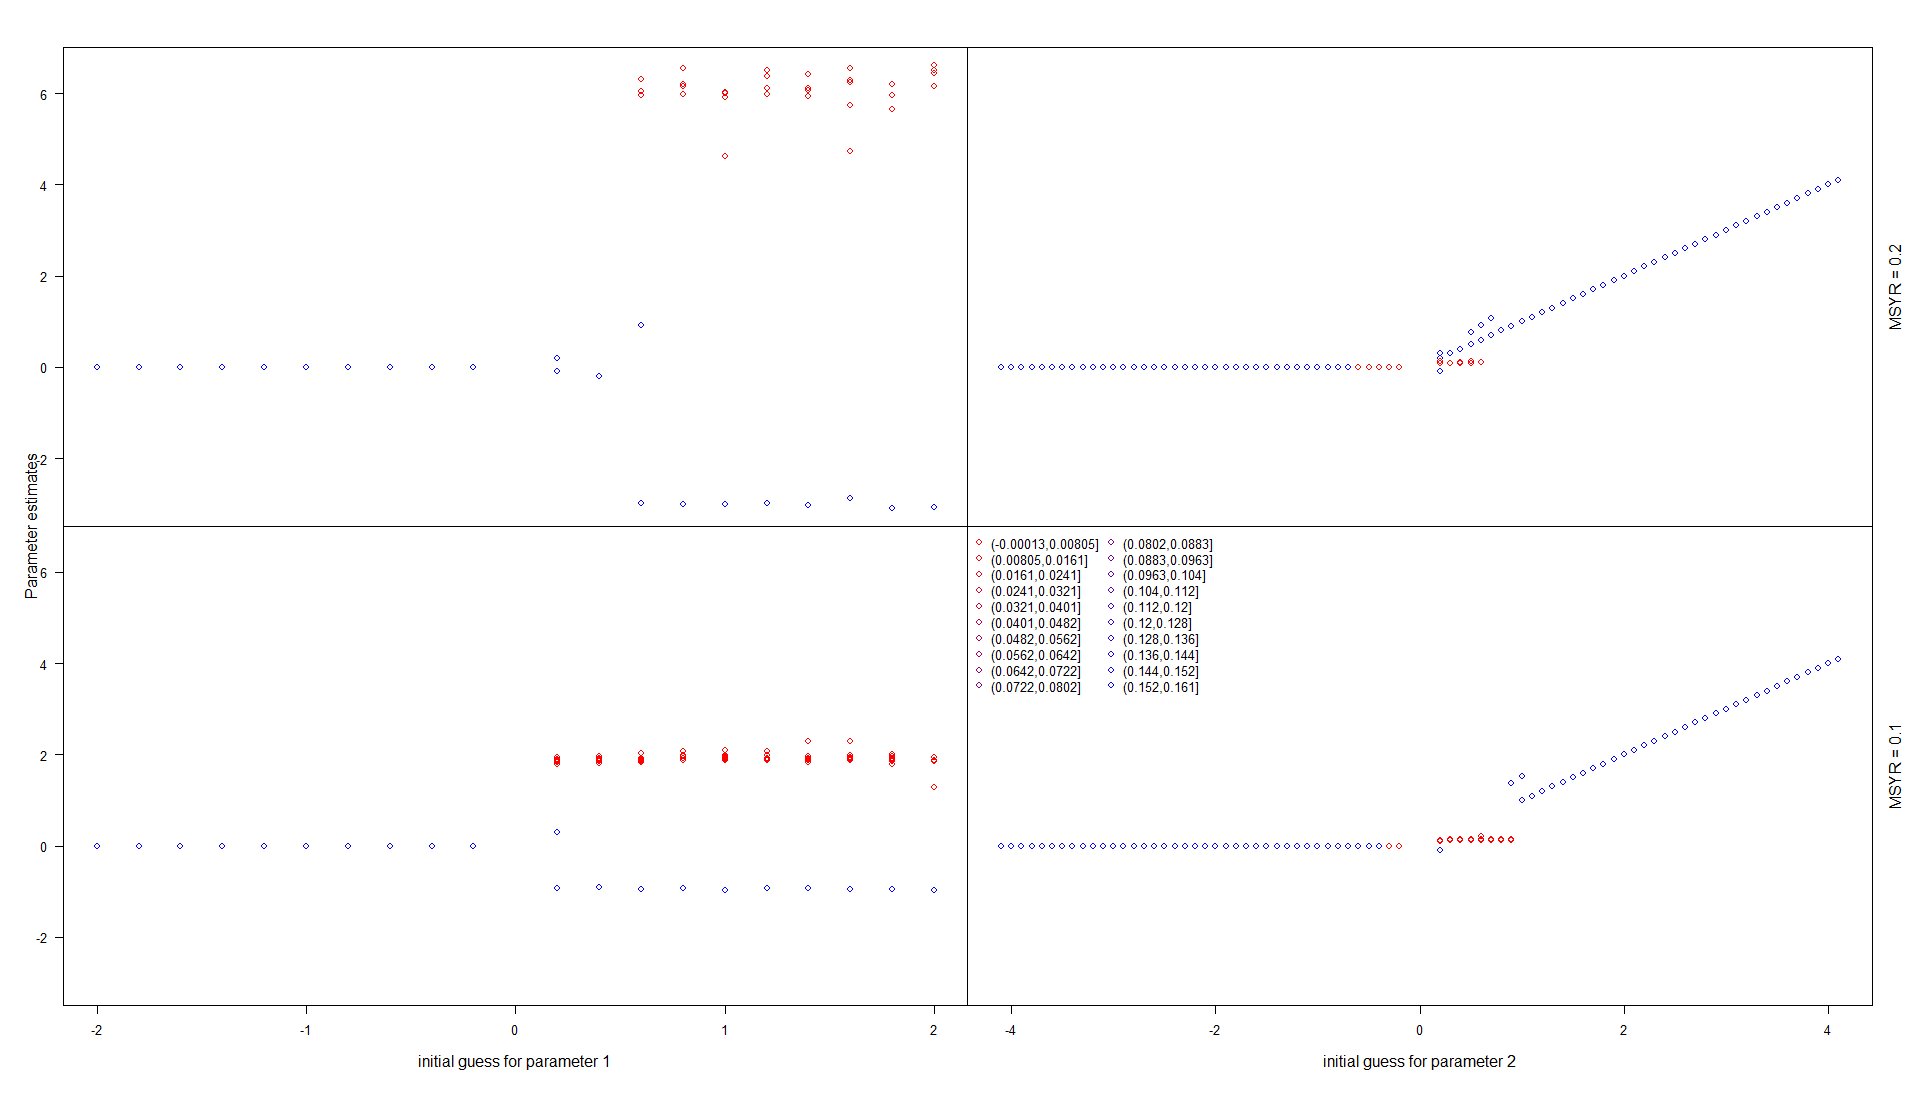
\includegraphics{c:/iwccla/ms/image.png}
\caption{Response curves for the base-case trials.}
\label{fig:respcurv_base}
\end{figure}

\subsubsection{References}\label{references}
% \bibliography{references}
%     \bibliographystyle{plain}

\end{document}
